% Options for packages loaded elsewhere
\PassOptionsToPackage{unicode}{hyperref}
\PassOptionsToPackage{hyphens}{url}
\PassOptionsToPackage{dvipsnames,svgnames*,x11names*}{xcolor}
%
\documentclass[
  12pt,
]{article}
\usepackage{lmodern}
\usepackage{amssymb,amsmath}
\usepackage{ifxetex,ifluatex}
\ifnum 0\ifxetex 1\fi\ifluatex 1\fi=0 % if pdftex
  \usepackage[T1]{fontenc}
  \usepackage[utf8]{inputenc}
  \usepackage{textcomp} % provide euro and other symbols
\else % if luatex or xetex
  \usepackage{unicode-math}
  \defaultfontfeatures{Scale=MatchLowercase}
  \defaultfontfeatures[\rmfamily]{Ligatures=TeX,Scale=1}
\fi
% Use upquote if available, for straight quotes in verbatim environments
\IfFileExists{upquote.sty}{\usepackage{upquote}}{}
\IfFileExists{microtype.sty}{% use microtype if available
  \usepackage[]{microtype}
  \UseMicrotypeSet[protrusion]{basicmath} % disable protrusion for tt fonts
}{}
\makeatletter
\@ifundefined{KOMAClassName}{% if non-KOMA class
  \IfFileExists{parskip.sty}{%
    \usepackage{parskip}
  }{% else
    \setlength{\parindent}{0pt}
    \setlength{\parskip}{6pt plus 2pt minus 1pt}}
}{% if KOMA class
  \KOMAoptions{parskip=half}}
\makeatother
\usepackage{xcolor}
\IfFileExists{xurl.sty}{\usepackage{xurl}}{} % add URL line breaks if available
\IfFileExists{bookmark.sty}{\usepackage{bookmark}}{\usepackage{hyperref}}
\hypersetup{
  pdftitle={Brother, Can You Spare a Manufacturing Job? How Voters React to Deindustrialization},
  pdfauthor={Catherine Darin and Zagreb Mukerjee},
  colorlinks=true,
  linkcolor=Maroon,
  filecolor=Maroon,
  citecolor=Blue,
  urlcolor=red,
  pdfcreator={LaTeX via pandoc}}
\urlstyle{same} % disable monospaced font for URLs
\usepackage[margin=1in]{geometry}
\usepackage{graphicx,grffile}
\makeatletter
\def\maxwidth{\ifdim\Gin@nat@width>\linewidth\linewidth\else\Gin@nat@width\fi}
\def\maxheight{\ifdim\Gin@nat@height>\textheight\textheight\else\Gin@nat@height\fi}
\makeatother
% Scale images if necessary, so that they will not overflow the page
% margins by default, and it is still possible to overwrite the defaults
% using explicit options in \includegraphics[width, height, ...]{}
\setkeys{Gin}{width=\maxwidth,height=\maxheight,keepaspectratio}
% Set default figure placement to htbp
\makeatletter
\def\fps@figure{htbp}
\makeatother
\setlength{\emergencystretch}{3em} % prevent overfull lines
\providecommand{\tightlist}{%
  \setlength{\itemsep}{0pt}\setlength{\parskip}{0pt}}
\setcounter{secnumdepth}{-\maxdimen} % remove section numbering
\usepackage{bm}
\usepackage{booktabs}
\usepackage{longtable}
\usepackage{array}
\usepackage{multirow}
\usepackage{wrapfig}
\usepackage{float}
\usepackage{colortbl}
\usepackage{pdflscape}
\usepackage{tabu}
\usepackage{threeparttable}
\usepackage{threeparttablex}
\usepackage[normalem]{ulem}
\usepackage{makecell}
\usepackage{xcolor}

\title{Brother, Can You Spare a Manufacturing Job? How Voters React to
Deindustrialization}
\author{Catherine Darin and Zagreb Mukerjee}
\date{11/29/2021}

\begin{document}
\maketitle

\renewcommand{\arraystretch}{1.1}
\renewcommand{\topfraction}{.85}
\renewcommand{\bottomfraction}{.7}
\renewcommand{\textfraction}{.15}
\renewcommand{\floatpagefraction}{.66}
\setcounter{topnumber}{3}
\setcounter{bottomnumber}{3}
\setcounter{totalnumber}{4}

\hypertarget{r-includefalse-optionstinytex.verbose-true}{%
\section{\texorpdfstring{\texttt{\{r,\ include=FALSE\}\ \#\ options(tinytex.verbose\ =\ TRUE)\ \#}}{\{r, include=FALSE\} \# options(tinytex.verbose = TRUE) \#}}\label{r-includefalse-optionstinytex.verbose-true}}

\hypertarget{replication-instructions}{%
\subsection{Replication Instructions}\label{replication-instructions}}

Please find instructions and relevant code to replicate our analysis
here: \url{https://github.com/zagrebmukerjee/ReplicationPaper}

\hypertarget{introduction}{%
\subsection{Introduction}\label{introduction}}

What led to Donald Trump's surprising 2016 election victory? This paper
examines the potential contribution of deindustrialization. Counties
differ by exposure to manufacturing, which we use in an
instrumental-variable approach to identify the effect of manufacturing
job loss on change in Democratic vote share. We find that Democratic
vote share falls in counties with high manufacturing job loss since
2004. Disaggregating this result by race shows that the Democratic vote
share fell where layoffs affected white populations, and rose where
layoffs affected nonwhites. This suggests a racial component to how
voters process economic hardship.

Base paper: Baccini and Weymouth 2021, ``Gone For Good:
Deindustrialization, White Voter Backlash, and US Presidential Voting.''
\emph{APSR}.

\hypertarget{outline}{%
\subsection{Outline}\label{outline}}

\hypertarget{framing-story}{%
\paragraph{Framing story}\label{framing-story}}

To do: Qualitative description of the trajectory of XYZ county that
swung from Obama to Trump and suffered big manufacturing layoffs. This
will establish the stakes and connect this to the broader conversation.

\hypertarget{substantive-importance}{%
\subsubsection{Substantive importance}\label{substantive-importance}}

Why did Trump win in 2016? There is a longstanding debate about relative
importance of race and economic factors. Complicated by the interaction
of the two. We hope to identify the importance of manufacturing job
losses, both in aggregate and for different racial groups. Eventually we
think that people should stop asking ``race or economics'' when the
answer is likely both.

\hypertarget{empirical-strategy}{%
\subsubsection{Empirical strategy}\label{empirical-strategy}}

Differential manufacturing exposure across counties allows for
identification of the causal effect of deindustrialization on change in
Dem vote share. Further differences in racial exposure to mfg layoffs
allows for identification of the interaction between race and
deindustrialization.

\hypertarget{data-and-methods}{%
\subsubsection{Data and methods}\label{data-and-methods}}

Data is Census Quarterly Workforce Indicators, which break down county
employment by industry, race and ethnicity. Augmented with public data
on vote shares, employment, etc.

We look at total employment and manufacturing employment (NAICS 31-33,
see extensions below). We then compute net change in mfg jobs (long term
job loss) from 2004 to 2015, relative to employment in 2004.

We might be worried about endogeneity for manufacturing job losses. So
we use a shift-share instrument: we predict net job losses per worker
with county-level manufacturing as a share of total employment, plus
controls.

Controls: unemployment in 2015, college educated share of population,
male share of population, layoffs in service sector, white share of
population (to control for demographic trends). We want to know if
there's something singular about manufacturing jobs.

\hypertarget{extension-relative-to-baccini-and-weymouth-2021}{%
\subsubsection{Extension Relative to Baccini and Weymouth
(2021)}\label{extension-relative-to-baccini-and-weymouth-2021}}

In their main model, Baccini and Weymouth looked at the effect of gross
manufacturing job losses from 2012 to 2015 on the change in Democratic
vote share in the 2016 presidential election.

Our key extension of Baccini and Weymouth's analysis is changing the
quantity of interest from \textbf{gross} manufacturing job losses to
\textbf{net} manufacturing job losses. For example, in Baccini and
Weymouth's model, if a county lost 400 manufacturing jobs from 2012-2015
and also gained 400 manufacturing jobs over the same period, they would
count 400 overall layoffs. Using our measure of \emph{net} manufacturing
job losses, we would consider this example a 0 net change in
manufacturing employment. Given that job destruction and creation is a
natural dynamic within the economy (i.e.~seasonal employment, creative
destruction), we think that \emph{net} job losses is a more meaningful
measure.

Using \emph{net} manufacturing job losses as our outcome, we replicate
Baccini and Weymouth's main model, which uses 2012-2015 manufacturing
(gross) job losses to explain the change in Democratic vote share in
2016. Using their specifications, we find totally opposite results -
that a \emph{net} increase in white manufacturing jobs \emph{increased}
Democratic vote share, while a \emph{net} increase in non-white
manufacturing jobs \emph{decreased} Democratic vote share. (See Table 3)

However, we don't think this is capturing the important dynamic at play.
From 2012 to 2015, the national economy experienced a net increase in
manufacturing jobs following the 2008 recession (See Figure 1). During
this time of recovery, counties that experienced the most pronounced
manufacturing job losses in prior years were also likely to experience
the most pronounced recovery. Because of this v-shaped recovery,
focusing only on 2012-2015 job losses/gains paints a distorted picture.
{[}To DO: Empirically show negative correlation described here{]}

If we expand our measure of net manufacturing job losses to include the
2004 to 2011 period - which covers most of the period when the U.S.
manufacturing economy was hit most intensely (See Figure 1) -- we get a
result that corroborates the core intuition of Baccini and Weymouth (See
Table 4). That is, we find that net white manufacturing job losses
decreased Democratic vote share, while net non-white manufacturing job
losses increased Democratic vote share.

It is important to highlight the substantive importance of the
\emph{timing} of manufacturing layoffs on political outcomes. Whereas
Baccini and Weymouth's analysis suggests that economic changes lead to
immediate political consequences, our analysis shows that economic
changes can have lagged and variable effects on political outcomes. The
mechanisms of these lagged effects merit further study.

{[}Note: to demonstrate our point about \textbf{variable} effects, In
our next iteration of the analysis, we will show that manufacturing job
losses had little explanatory effect on changes in Democratic vote share
in other elections (2012 and 2020).{]}

\hypertarget{key-findings}{%
\subsubsection{Key Findings}\label{key-findings}}

We find that, in aggregate, manufacturing job losses were associated
with loss of Democratic vote share in the 2016 election. 10
manufacturing job losses per worker in a county since 2004 corresponded
to a 3.8 \% loss in vote share, plus or minus 3.3 \%. Breaking it down
by race, we see that {[}TO DO: complete thought{]}.

Figure 3 demonstrates the practical significance of our estimates. Using
our main results from regression 3 in Table 4, we simulate a
counterfactual 2016 election assuming that all counties experienced
white manufacturing job losses equivalent to the county at the 25th
national percentile. We highlight states in purple if this
counterfactual shows a state flipping from Trump to Clinton.

Additionally, we find that, given the evolution of the business cycle,
considering only recent job losses can paint a misleading picture of the
relationship between manufacturing job losses and changes in vote share.
In fact, we find that net manufacturing job losses from 2004 to 2011 are
crucial to explaining Trump's 2016 win. This finding suggests that
economic changes, like manufacturing layoffs, can have lagged and
variable political consequence.

\hypertarget{potential-future-work}{%
\subsubsection{Potential Future Work}\label{potential-future-work}}

\begin{itemize}
\tightlist
\item
  Temporal: Finding a better way to characterize the potentially lagged
  effect of manufacturing job losses on Democratic votes. Incorporating
  study of the 2008, 2012, 2020 elections.
\item
  Disaggregation: Instead of instrumenting by manufacturing share,
  perhaps we can look at layoffs by industry in each county. While
  aggregate manufacturing employment may be endogenous, there's less
  reason to believe that specific industries would be (cf.~Autor, Dorn
  and Hanson). This may also allow us to get further away from
  ecological inference problems.
\item
  Trend-cycle estimation: There are techniques from econometrics and
  other places that could potentially be used to decompose gross layoffs
  into seasonal and non-seasonal components.
\item
  Mechanisms: survey work to examine where the racial difference in
  economic voting behavior comes from. Is it expressive? Is it because
  information is transmitted along racially segregated networks?
\end{itemize}

\hypertarget{tables-and-figures}{%
\subsection{Tables and Figures}\label{tables-and-figures}}

\hypertarget{manufacturing-layoffs-over-time}{%
\subsubsection{Manufacturing Layoffs Over
Time}\label{manufacturing-layoffs-over-time}}

\begin{verbatim}
## Warning: Removed 2 rows containing missing values (position_stack).
\end{verbatim}

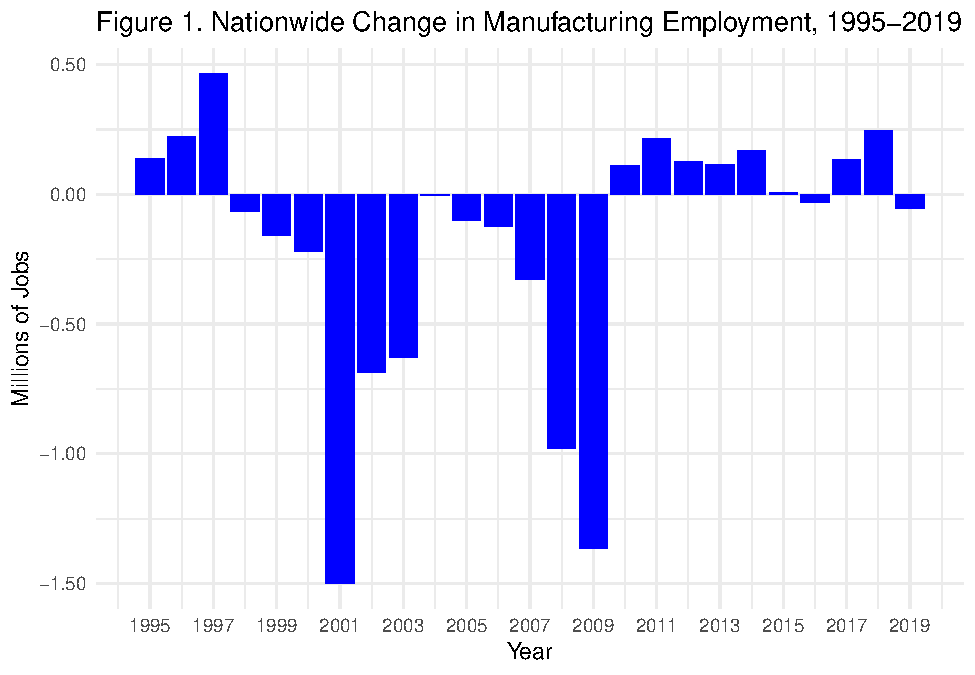
\includegraphics{Draft_files/figure-latex/unnamed-chunk-1-1}

\newpage

\hypertarget{geographic-concentration-of-layoffs}{%
\subsubsection{Geographic Concentration of
Layoffs}\label{geographic-concentration-of-layoffs}}

\hypertarget{to-15}{%
\subsubsection{04 to 15}\label{to-15}}

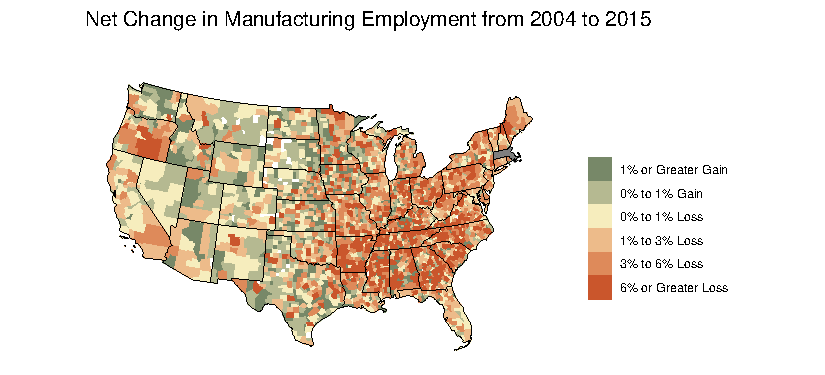
\includegraphics{Draft_files/figure-latex/unnamed-chunk-2-1}

\newpage

\hypertarget{to-15-1}{%
\subsubsection{12 to 15}\label{to-15-1}}

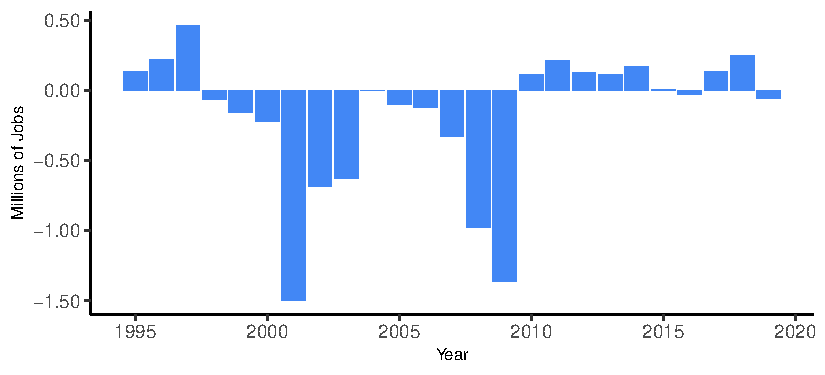
\includegraphics{Draft_files/figure-latex/unnamed-chunk-3-1}

\newpage

\hypertarget{descriptive-statistics}{%
\subsubsection{Descriptive Statistics}\label{descriptive-statistics}}

\begin{table}[!h]

\caption{\label{tab:unnamed-chunk-4}Manufacturing Job Changes 2004-2015}
\centering
\resizebox{\linewidth}{!}{
\begin{tabular}[t]{lrrrrr}
\toprule
  & Mean & Std Dev & 25th Pctile & Median & 75th Pctile\\
\midrule
Mfg Share of Emp & 0.20 & 0.15 & 0.09 & 0.17 & 0.29\\
Mfg Share of Emp (White) & 0.16 & 0.13 & 0.06 & 0.13 & 0.22\\
Mfg Share of Emp (Nonwhite) & 0.05 & 0.07 & 0.01 & 0.02 & 0.06\\
Change in Mfg Jobs/ Worker & 0.04 & 0.09 & -0.01 & 0.02 & 0.06\\
Change in Mfg Jobs/ Worker (W) & 0.03 & 0.07 & 0.00 & 0.02 & 0.06\\
\addlinespace
Change in Mfg Jobs/ Worker (NW) & 0.00 & 0.04 & -0.01 & 0.00 & 0.01\\
\bottomrule
\end{tabular}}
\end{table}

\begin{table}[!h]

\caption{\label{tab:unnamed-chunk-4}Manufacturing Job Changes 2012-2015}
\centering
\resizebox{\linewidth}{!}{
\begin{tabular}[t]{lrrrrr}
\toprule
  & Mean & Std Dev & 25th Pctile & Median & 75th Pctile\\
\midrule
Change in Dem Vote Share & -0.06 & 0.05 & -0.10 & -0.05 & -0.03\\
Mfg Share of Emp & 0.20 & 0.16 & 0.08 & 0.16 & 0.28\\
Mfg Share of Emp (White) & 0.15 & 0.13 & 0.06 & 0.12 & 0.22\\
Mfg Share of Emp (Nonwhite) & 0.05 & 0.07 & 0.01 & 0.03 & 0.06\\
Change in Mfg Jobs/ Worker & -0.01 & 0.05 & -0.02 & 0.00 & 0.01\\
\addlinespace
Change in Mfg Jobs/ Worker (W) & 0.00 & 0.03 & -0.01 & 0.00 & 0.01\\
Change in Mfg Jobs/ Worker (NW) & 0.00 & 0.02 & -0.01 & 0.00 & 0.00\\
\bottomrule
\end{tabular}}
\end{table}

\newpage

\hypertarget{regression-results-using-2004-2015-net-manu-job-change}{%
\subsubsection{Regression Results (Using 2004-2015 Net Manu Job
Change)}\label{regression-results-using-2004-2015-net-manu-job-change}}

\begin{table}[!htbp] \centering 
  \caption{Effect of Manufacturing Layoffs on Democratic Vote Share (since 2004)} 
  \label{} 
\begin{tabular}{@{\extracolsep{5pt}}lcccc} 
\\[-1.8ex]\hline 
\hline \\[-1.8ex] 
 & \multicolumn{4}{c}{\textit{Dependent variable:}} \\ 
\cline{2-5} 
\\[-1.8ex] & \multicolumn{4}{c}{Change in Share (2016-2012)} \\ 
\\[-1.8ex] & (1) & (2) & (3) & (4)\\ 
\hline \\[-1.8ex] 
 Manufacturing Layoffs & $-$0.34$^{**}$ & $-$0.38$^{**}$ &  &  \\ 
  & (0.14) & (0.17) &  &  \\ 
  & & & & \\ 
 White Manufacturing Layoffs &  &  & $-$0.23$^{***}$ & $-$0.32$^{***}$ \\ 
  &  &  & (0.08) & (0.10) \\ 
  & & & & \\ 
 Nonwhite Manufacturing Layoffs &  &  & 0.15$^{***}$ & 0.20$^{***}$ \\ 
  &  &  & (0.05) & (0.06) \\ 
  & & & & \\ 
\hline \\[-1.8ex] 
Controls For White Share/Service Layoffs & No & Yes & No & Yes \\ 
Observations & 3,049 & 3,049 & 2,750 & 2,750 \\ 
Adjusted R$^{2}$ & 0.72 & 0.72 & 0.75 & 0.75 \\ 
\hline 
\hline \\[-1.8ex] 
\textit{Note:}  & \multicolumn{4}{r}{$^{*}$p$<$0.1; $^{**}$p$<$0.05; $^{***}$p$<$0.01} \\ 
\end{tabular} 
\end{table}

\newpage

\hypertarget{regression-results-using-2012-2015-net-manu-job-change}{%
\subsubsection{Regression Results (Using 2012-2015 Net Manu Job
Change)}\label{regression-results-using-2012-2015-net-manu-job-change}}

\begin{table}[!htbp] \centering 
  \caption{Effect of Manufacturing Layoffs on Democratic Vote Share} 
  \label{} 
\begin{tabular}{@{\extracolsep{5pt}}lcccc} 
\\[-1.8ex]\hline 
\hline \\[-1.8ex] 
 & \multicolumn{4}{c}{\textit{Dependent variable:}} \\ 
\cline{2-5} 
\\[-1.8ex] & \multicolumn{4}{c}{Change in Share (2012-2016)} \\ 
\\[-1.8ex] & (1) & (2) & (3) & (4)\\ 
\hline \\[-1.8ex] 
 Manufacturing Layoffs & 0.43$^{**}$ & 0.37$^{**}$ &  &  \\ 
  & (0.17) & (0.17) &  &  \\ 
  & & & & \\ 
 White Manufacturing Layoffs &  &  & 6.50$^{***}$ & 2.33$^{***}$ \\ 
  &  &  & (2.20) & (0.76) \\ 
  & & & & \\ 
 Nonwhite Manufacturing Layoffs &  &  & $-$3.99$^{***}$ & $-$1.42$^{***}$ \\ 
  &  &  & (1.36) & (0.47) \\ 
  & & & & \\ 
\hline \\[-1.8ex] 
Controls For White Share/Service Layoffs & No & Yes & No & Yes \\ 
Observations & 3,064 & 3,064 & 2,765 & 2,765 \\ 
Adjusted R$^{2}$ & 0.73 & 0.73 & 0.75 & 0.75 \\ 
\hline 
\hline \\[-1.8ex] 
\textit{Note:}  & \multicolumn{4}{r}{$^{*}$p$<$0.1; $^{**}$p$<$0.05; $^{***}$p$<$0.01} \\ 
\end{tabular} 
\end{table}

\newpage

\hypertarget{counterfactual-assessment-of-election-using-2004-2015-layoffs}{%
\subsubsection{Counterfactual assessment of election (Using 2004-2015
Layoffs)}\label{counterfactual-assessment-of-election-using-2004-2015-layoffs}}

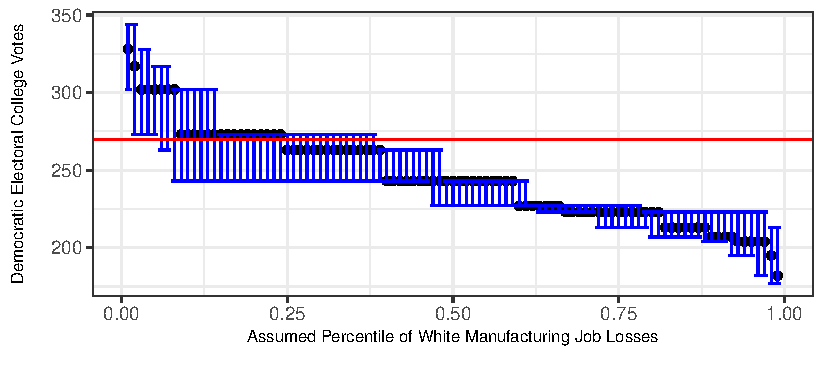
\includegraphics{Draft_files/figure-latex/unnamed-chunk-7-1}

\end{document}
